\documentclass{beamer}


\usepackage{pgfpages}
%\setbeameroption{show notes}
%\setbeameroption{show notes on second screen=right}
\mode<presentation> {
  \usetheme{Warsaw}
  % ou autre ...

  \setbeamercovered{transparent}
  % ou autre chose (il est également possible de supprimer cette ligne)
}


\usepackage[spanish,es-tabla]{babel}
\usepackage[utf8]{inputenc}
\usepackage{times}
\usepackage[T1]{fontenc}
\usepackage{tikz}
\usepackage{makecell}
\usepackage{fancyvrb}
\usepackage{listings}
\usepackage{pgfplots}
\usetikzlibrary{pgfplots.statistics}
\pgfdeclareimage[height=0.5cm]{le-logo}{logo-usb}
\logo{\pgfuseimage{le-logo}}
\setbeamertemplate{footline}[frame number]

\renewcommand{\lstlistingname}{Fragmento de Código}
\renewcommand{\lstlistlistingname}{Índice de Fragmentos de Código}
\lstset{
	basicstyle=\ttfamily\footnotesize,
	frame=single,
	captionpos=b,
	numbers=left,
	showstringspaces=false,
	aboveskip=1em,
	belowskip=2em,
	xleftmargin=1em,
	xrightmargin=1em,
	tabsize=4}


%%%%%%%%%%%%%%%%%%%%%%%%%%%
\title{Sistema de Recomendación de Soluciones a Errores de Programación en Lenguaje C usando Minería de Datos}
%\subtitle{PROYECTO DE GRADO}

\author{Christhian Guevara\inst{1} \and Masun Nabhan Homsi\inst{2}}

\institute{\inst{1}AUTOR\\ \inst{2}TUTOR\\ ~\\ Coordinación de Ingeniería de la Computación\\  Universidad Simón Bolívar}

\date{Sartenejas, Enero~de~2019}

\begin{document}


\begin{frame}
  \titlepage
\end{frame}

\begin{frame}{Contenido}
  \tableofcontents
\end{frame}

\section{Introducción}

\subsection*{Síntesis}
\begin{frame}{Síntesis}
\begin{center}
Desarrollar Software => Solucionar Errores
\end{center}
\begin{block}{Bugs}
Son errores de comprensión o lógica, e incluso comportamientos no definidos o inesperados.
\end{block}
\begin{center}
19\% del tiempo se invierte en consultar fuentes externas.
\end{center}
Algunas fuentes externas son:
  \begin{itemize}
  \item Foros
  \item Listas de Correo Electrónico
  \item Sitios de Preguntas y Respuestas
  \end{itemize}
\end{frame}

\begin{frame}{Síntesis}
Problemas del Proceso de Búsqueda:
  \begin{itemize}
  \item Falta de automatización
  \item Se requiere habilidad para formular la consulta
  \item La consulta no guarda relación con el código
  \end{itemize}
  
\begin{center}
``Los motores de busqueda son ineficaces para realizar consultas empleando el código fuente''.
\end{center}
\end{frame}

\subsection{Planteamiento del Problema}
\begin{frame}{Planteamiento del Problema}
El proceso de solucionar errores es repetitivo y tedioso, en consecuencia:
\begin{itemize}
  \item Requiere consultar fuentes externas con frecuencia
  \item No se emplea el código fuente en la consulta
  \item Se debe describir el problema e identificar su origen
  \item La documentación generalmente es escasa, incomprensible o inexistente.
\end{itemize}
\begin{center}
=> Impide encontrar solución al problema en tiempo razonable y pospone la realización de la tarea asignada.
\end{center}
\end{frame}

\subsection*{Antecedentes}
\begin{frame}{Antecedentes}
\begin{center}
Trabajos previos en el área apuntan a desarrollar un Sistema de Recomendación que
se beneficie del conocimiento provisto por la comunidad de Stack Overflow.
\end{center}
Algunas de estas investigaciones son:
\begin{description}
  \item[Debugging with the Crowd] presenta un Sistema de Recomendación como una herramienta para \textit{debugging}.
  \item[Prompter] es un Sistema de Recomendación que se muestra como un \textit{plug-in} para \textit{Eclipse IDE}.
  \item[PDE4Java] es un motor para detección de documentos similares en \textit{Java}.
\end{description}
\end{frame}

\subsection{Justificación}
\begin{frame}{Justificación}
Muchos de los problemas que afectan el desarrollo de software se relacionan directamente con el proceso de búsqueda.
El programador invierte tiempo valioso y sus consultas no suelen ser exitosas.

\begin{center}
``Queda en evidencia la falta de herramientas que faciliten el proceso de búsqueda al desarrollador''.
\end{center}
\end{frame}

\subsection{Objetivos}
\begin{frame}{Objetivos}
\textbf{Objetivo General}


\begin{center}
Desarrollar un sistema capaz de recomendar soluciones a errores cometidos por el programador en lenguaje C,
apoyándose sobre algoritmos de Minería de Datos.
\end{center}
\end{frame}

\begin{frame}{Objetivos}
\textbf{Objetivos Específicos}

\begin{itemize}
  \item Aplicar algoritmos de minería de datos para explotar los conocimientos
  de programación en lenguaje c de la comunidad de programadores del sitio web \textit{Stack Overflow}.
  
  \item Implementar una herramienta que ayude al programador a identificar errores en el código,
  mediante una lista de recomendaciones de posibles soluciones proporcionada por la comunidad.

  \item Establecer un modelo de clasificación que incluya aspectos relacionados
  a la reputación de los usuarios de \textit{Stack Overflow}.
\end{itemize}
\end{frame}

\section{Marco Teórico}
\subsection{Minería de Datos}
\begin{frame}{Minería de Datos}
El objetivo general del proceso de minería de datos consiste en extraer
información de una fuente de datos e intentar convertir esa información
en un conjunto aprovechable de conocimientos.

~

Proceso que consiste de 3 pasos:
\begin{itemize}
  \item Preprocesamiento.
  \item Análisis.
  \item Interpretación.
\end{itemize}
\end{frame}

\subsection{Similitud entre Documentos}
\begin{frame}{Similitud entre Documentos}
Es un subárea de minería de datos que aborda el problema de encontrar
documentos similares.

~

Ampliamente utilizado en:
\begin{itemize}
  \item Detección de Plagio.
  \item Detección de Clones.
\end{itemize}

~

A su vez, involucra el análisis del código fuente.
\end{frame}

\begin{frame}{Similitud entre Documentos}
Posibles variaciones en el código fuente:
\begin{itemize}
  \item cambio de formato
  \item cambio de identificadores
  \item cambio en el orden de los operandos en las expresiones
  \item cambio del tipo de datos
  \item sustitución de expresiones por sus equivalentes
  \item introducción de declaraciones redundantes
  \item cambio en el orden de declaraciones
  \item cambio en la estructura de las instrucciones de iteración
  \item cambio en la estructura de las declaraciones de selección
  \item sustitución de las llamadas a función por el cuerpo
  \item introducción de declaraciones no estructuradas
  \item combinación del código original y copiado
  \item traducción del código de un lenguaje a otro
\end{itemize}
\end{frame}

\begin{frame}{Similitud entre Documentos}
Clasificación del código fuente por similitud:
\begin{description}
  \item [Tipo I] Idénticos exceptuando las variaciones en espacios, diseño y comentarios.
  \item [Tipo II] Sintácticamente idénticos exceptuando las variaciones en identificadores, literales, tipos, diseño y comentarios.
  \item [Tipo III] Con modificaciones adicionales. Expresiones alteradas y variaciones en identificadores, literales, tipos, diseño y comentarios.
  \item [Tipo IV] Que realizan el mismo cálculo pero son implementados a través de diferentes variantes sintácticas.
\end{description}
\end{frame}

\begin{frame}{Similitud entre Documentos}
Clasificación general de los métodos desarrollados:
\begin{itemize}
  \item Comparación basada en texto
  \item Comparación basada en lexemas
  \item Comparación basada en arboles de sintaxis
  \item Comparación basada en grafos de dependencia
  \item Comparación basada en métricas
  \item Comparación empleando enfoques híbridos
\end{itemize}
\end{frame}

\subsection{Document Fingerprinting}
\begin{frame}{Document Fingerprinting}
\begin{center}
``Es una técnica para la detección precisa de copias completas y parciales entre documentos''.
\end{center}

Consiste en dividir el texto en subsecuencias, calcular el \textit{hash} para cada 
subsecuencia y crear la firma a partir de éstos.

~
\begin{description}
  \item [Secuencia de ejemplo] pablito clavó un clavito
  \item [Secuencia de \textit{4-grams}] pabl abli blit lito itoc toca ocav cavo \\~~~~~~~~~~~ avou voun ounc uncl ncla clav lavi avit vito
  \item [Secuencia de \textit{hashes}] 77 72 43 19 91 50 17 98 8 88 67 39 78 7 \\~~~~~~~~~~~~~~~~~~~~~~~~~~~~~~~~~~~~~~~ 42 11 92
\end{description}
\end{frame}


\begin{frame}{Document Fingerprinting}
\textbf{Similitud}

Se puede medir la similitud empleando el coeficiente de similitud de \textit{Jaccard},
para ello, los elementos del conjunto serán aquellos valores de \textit{hash} que son calculados a partir del documento.

~
\begin{equation*}
J(A, B) = \frac{|A \cap B|}{|A \cup B|}
\end{equation*}
\end{frame}

\begin{frame}{Document Fingerprinting}
\textbf{Firma}

La firma se puede crear empleando la técnica de \textit{MinHash},
que sirve para estimar de forma eficiente el coeficiente de similitud de \textit{Jaccard}.

~

\textbf{MinHash}

Se selecciona un tamaño para la firma, 
se escoge igual cantidad de funciones de \textit{hash} universales,
se asocia una función a cada casilla y
se escoge el mínimo valor obtenido al aplicar la función correspondiente al conjunto de valores.
\end{frame}

\begin{frame}{Document Fingerprinting}
\textbf{Índice Invertido}

El \textit{Locality-Sensitive Hashing} es una técnica que se comporta de forma similar a un índice invertido,
permite realizar búsquedas sobre las firmas generadas mediante el \textit{MinHash}.

~

\textbf{Locality-Sensitive Hashing}

El enfoque general para el \textit{LSH},
consiste en emplear diversas funciones de \textit{hash} para asociar
los elementos de un conjunto a distintas ‘casillas’.
De esta manera, los elementos similares entre sí,
tienen mayores probabilidades de ser agrupados en las mismas ‘casillas’,
que los demás elementos.
Luego, se considera como ‘par candidato’
a cualquier par de elementos que se encuentre en la misma ‘casilla’
\end{frame}



\section{Marco Tecnológico}
\subsection*{Herramientas}
\begin{frame}{Herramientas}
\begin{columns}[T]

\column{.27\textwidth} % Left column and width
\begin{center}
\textbf{IDE}
\end{center}
\begin{figure}

\includegraphics[width=0.8\linewidth]{logo-eclipse}
\end{figure}

\column{.27\textwidth} % Right column and width
\begin{center}
\textbf{Extensiones}

~

Java

C/C++

Plug-in
\end{center}
\column{.27\textwidth} % Right column and width
\begin{center}
\textbf{Librerías}

~

CDT: CORE

Apache Commons Text
\end{center}
\end{columns}

~

~

\begin{columns}[T]

\column{.4\textwidth} % Left column and width
\begin{center}
\textbf{Base de Datos}
\begin{figure}

\includegraphics[width=0.37\linewidth]{logo-psql}
\end{figure}
\end{center}
\column{.4\textwidth} % Right column and width
\begin{center}
\textbf{Extensiones}

PL/pgSQL
\end{center}
\end{columns}
\end{frame}

\section{Marco Metodológico}
\subsection*{Metodología}
\begin{frame}{Esquema Metodológico}
\begin{figure}
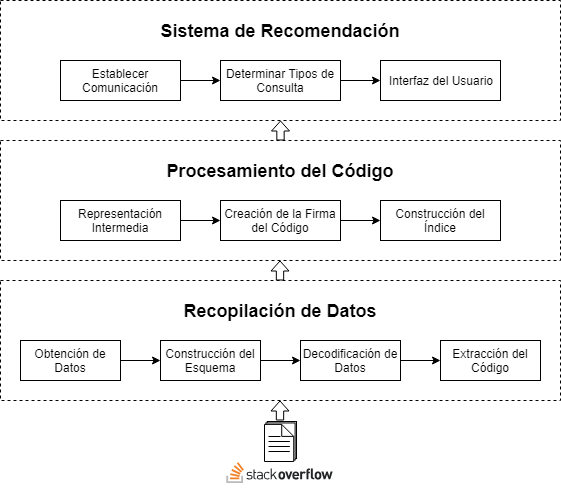
\includegraphics[width=0.6\linewidth]{metodo}
\end{figure}
\end{frame}

\section{Resultados}
\subsection{Recopilación de Datos}
\begin{frame}{Recopilación de Datos}
\begin{table}[h]
\caption{Cantidad de tópicos por etiqueta.}
\centering
\begin{tabular}{ccccc}
\hline
{Etiqueta} & {Preguntas} & {Respuestas} & \makecell{Respuestas\\Aceptadas} & {Total} \\
\hline
{todas} & $7.990.786$ & $13.684.117$ & $4.596.859$ & $21.736.593$ \\ 
{c/c++} & $442.450$ & $978.214$ & $284.297$ & $1.420.664$ \\ 
{c++} & $314.869$ & $684.362$ & $203.447$ & $999.231$ \\ 
{c} & $151.856$ & $362.244$ & $96.949$ & $514.100$ \\
\hline
\end{tabular}
\end{table}
\end{frame}

\begin{frame}{Recopilación de Datos}
\begin{table}[h]
\caption{Tópicos relacionados con c/c++.}
\centering
\begin{tabular}{cccc}
\hline
{Descripción} & {Preguntas} & {Respuestas} & {Total} \\
\hline
{todos} & $442.450$ & $978.214$ & $1.420.664$ \\ 
{con código} & $314.247$ & $459.073$ & $773.320$ \\ 
{relación} & $71.02\%$ & $46.93\%$ & $54.43\%$ \\
\hline
\end{tabular}
\end{table}
\begin{table}[h]
\caption{Cantidad de fragmentos de código}
\centering
\begin{tabular}{cccc}
\hline
{Descripción} & {Preguntas} & {Respuestas} & {Total} \\
\hline
{fragmentos} & $598.775$ & $778.940$ & $1.377.716$ \\
{relación} & $43.46\%$ & $56.54\%$ & $100.0\%$ \\
\hline
\end{tabular}
\end{table}
\end{frame}

\begin{frame}{Recopilación de Datos}
\begin{figure}[h]
\centering
\begin{tikzpicture}[scale=0.8]
\begin{axis}[
boxplot/draw direction=y,
x=2cm,
xtick={1,2,3},
xticklabels={Total, Preguntas, Respuestas},
]
\addplot+ [boxplot prepared={
lower whisker=0,
lower quartile=0,
median=1,
upper quartile=1,
upper whisker=2}
%average=1},
] coordinates {};
\addplot+ [boxplot prepared={
lower whisker=0,
lower quartile=0,
median=1,
upper quartile=2,
upper whisker=4}
%average=1},
] coordinates {};
\addplot+ [boxplot prepared={
lower whisker=0,
lower quartile=0,
median=0,
upper quartile=1,
upper whisker=2}
%average=0},
] coordinates {};
\end{axis}
\end{tikzpicture}
\caption{Estadísticas descriptivas de los fragmentos de código.}
\end{figure}
\end{frame}

\begin{frame}{Recopilación de Datos}
\begin{figure}[h]
\centering
\begin{tikzpicture}[scale=0.8]
\begin{axis}[
boxplot/draw direction=y,
x=2cm,
xtick={1,2,3},
xticklabels={Total, Preguntas, Respuestas},
]
\addplot+ [boxplot prepared={
lower whisker=1,
lower quartile=2,
median=5,
upper quartile=14,
upper whisker=31},
%upper whisker=1266},
] coordinates {};
\addplot+ [boxplot prepared={
lower whisker=1,
lower quartile=3,
median=8,
upper quartile=19,
upper whisker=42},
%upper whisker=1266},
] coordinates {};
\addplot+ [boxplot prepared={
lower whisker=1,
lower quartile=1,
median=4,
upper quartile=10,
upper whisker=23},
%upper whisker=1236},
] coordinates {};
\end{axis}
\end{tikzpicture}
\caption{Estadísticas descriptivas de las líneas de código.}
\end{figure}
\end{frame}

\subsection{Procesamiento del Código}
\begin{frame}[fragile]{Procesamiento del Código}
\textbf{Tópico ejemplo:}
\begin{lstlisting}[caption={Fragmento de código en c++}]
decimal trans = trackBar1.Value / 5000;
this.Opacity = trans;
\end{lstlisting}
\textbf{Lexemas identificados:}
\begin{Verbatim}[fontsize=\scriptsize]
 identifier, identifier, assign, identifier, dot, identifier, div,
integer, semi, identifier, dot, identifier, assign, identifier, semi
\end{Verbatim}

~

\textbf{Representación obtenida:}
\begin{Verbatim}[fontsize=\scriptsize]
          1, 1, 38, 1, 50, 1, 52, 2, 5, 1, 50, 1, 38, 1, 5
\end{Verbatim}
\end{frame}

\begin{frame}[fragile]{Procesamiento del Código}
\textbf{Secuencia de \textit{4-grams}:}
\begin{Verbatim}[fontsize=\scriptsize]
(1,1,38,1), (1,38,1,50), (38,1,50,1), (1,50,1,52), (50,1,52,2),
  (1,52,2,5), (52,2,5,1), (2,5,1,50), (5,1,50,1), (1,50,1,38),
                    (50,1,38,1), (1,38,1,5)
\end{Verbatim}

\textbf{Secuencia de \textit{hashes}:}
\begin{Verbatim}[fontsize=\scriptsize]
5328, 767281, 110488464, 1016115, 146320561, 1057684, 152306496,
    3068977, 11950992, 1016101, 146318544, 767236, 110482127
\end{Verbatim}

\begin{gather*}
firma(C_1) = (604227, 14244687, \dots, 17027248)
\end{gather*}
\end{frame}

\begin{frame}{Procesamiento del Código}
\begin{table}[h]
\caption{Configuración del \textit{MinHash}.}
\centering
\begin{tabular}{cc}
\hline
{Funciones} & {Error} \\
\hline
100 & $10.0\%$ \\ 
\hline
\end{tabular}
\end{table}
\begin{table}[h]
\caption{Configuración del \textit{LSH}.}
\centering
\begin{tabular}{ccc}
\hline
{Bandas} & {Filas} & {Umbral} \\
\hline
20 & 5 & $54.93\%$ \\ 
\hline
\end{tabular}
\end{table}
\end{frame}

\begin{frame}{Procesamiento del Código}
\textbf{Conjunto 1:}
\begin{table}[h]
\caption{Posición de los fragmentos de código.}
\centering
\begin{tabular}{ccc}
\hline
{Top1} & {Top10} & {Otro} \\
\hline
730 & 122 & 148 \\ 
\hline
\end{tabular}
\end{table}
\begin{table}[h]
\caption{Estadísticas generales.}
\centering
\begin{tabular}{cccc}
\hline
{T.Total} & {T.Consulta} & {P.Candidatos} & {E.Firma}\\
\hline
194\textit{ms} & 185\textit{ms} & 500 & $0.28$\textit{ms}\\ 
\hline
\end{tabular}
\end{table}
\end{frame}

\begin{frame}{Procesamiento del Código}
\textbf{Conjunto 2:}
\begin{table}[h]
\caption{Clasificación de Fragmentos de Código.}
\centering
\begin{tabular}{ccccc}
\hline
{Rango 1} & {Rango 2} & {Rango 3} & {Rango 4} & {Sin rango} \\
\hline
$12$ & $8$ & $20$ & $55$ & $100$ \\
\hline
\end{tabular}
\end{table}

~
\begin{description}
  \item [Rango 1] Estructuralmente iguales. Similitud >= 95\%.
  \item [Rango 2] Variaciones en los \textit{n-grams}. Similitud >= 85\%.
  \item [Rango 3] Cambios estructurales básicos. Similitud >= 70\%.
  \item [Rango 4] Cambios estructurales notables. Similitud >= 50\%.
  \item [Sin rango] Poca o ninguna similitud.
\end{description}
\end{frame}

\begin{frame}{Procesamiento del Código}
\begin{figure}[h]
\centering
\begin{tikzpicture}[scale=0.8]
\begin{axis}[
boxplot/draw direction=y,
x=2cm,
xtick={1,2,3,4,5},
xticklabels={Rango1, Rango2, Rango3, Rango4, SinRango},
]
\addplot+ [boxplot prepared={
lower whisker=2,
lower quartile=7,
median=8,
upper quartile=10.5,
upper whisker=15},
] coordinates {};
\addplot+ [boxplot prepared={
lower whisker=3,
lower quartile=7,
median=7.5,
upper quartile=10.5,
upper whisker=12},
] coordinates {};
\addplot+ [boxplot prepared={
lower whisker=4,
lower quartile=10,
median=12.5,
upper quartile=18.5,
upper whisker=23},
] coordinates {};
\addplot+ [boxplot prepared={
lower whisker=6,
lower quartile=15,
median=22,
upper quartile=31,
upper whisker=45},
] coordinates {};
\addplot+ [boxplot prepared={
lower whisker=1,
lower quartile=22.5,
median=31,
upper quartile=38,
upper whisker=51},
] coordinates {};
\end{axis}
\end{tikzpicture}
\caption{Estadísticas descriptivas de las líneas de código.}
\end{figure}
\end{frame}

\begin{frame}{Procesamiento del Código}
\begin{table}[h]
\caption{Clasificación de Fragmentos de Código en el rango $8\pm1$.}
\centering
\begin{tabular}{ccccc}
\hline
{Rango 1} & {Rango 2} & {Rango 3} & {Rango 4} & {Sin rango} \\
\hline
$6$ & $4$ & $3$ & $1$ & $2$ \\
$37.5\%$ & $25.0\%$ & $18.75\%$ & $6.25\%$ & $12.5\%$ \\
\hline
\end{tabular}
\end{table}
\end{frame}

\subsection{Sistema de Recomendación}
\begin{frame}{Estructura de Comunicación}
\begin{figure}
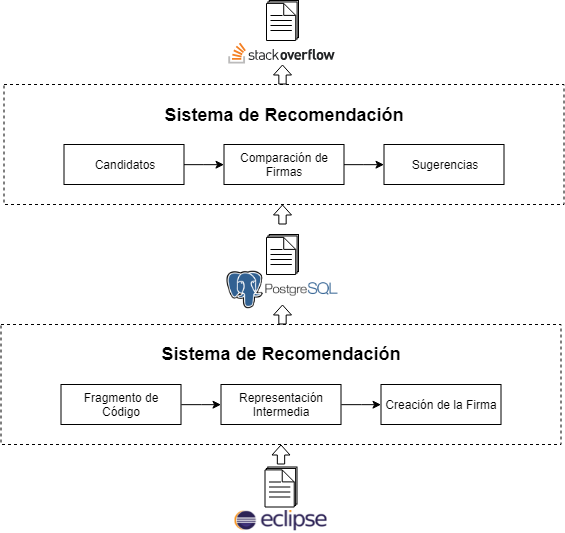
\includegraphics[width=0.6\linewidth]{comunicacion}
\end{figure}
\end{frame}

\begin{frame}{Filtros de Consulta}
\begin{columns}[T]

\column{.27\textwidth} % Left column and width
\begin{center}
\textbf{Tipo\\~}

~

-

Pregunta

Respuesta
\end{center}

\column{.27\textwidth} % Right column and width
\begin{center}
\textbf{Respuesta Aceptada}

~

-

SI
\end{center}
\column{.27\textwidth} % Right column and width
\begin{center}
\textbf{Rango\\~}

~

-

1

2

3

4
\end{center}
\end{columns}
\end{frame}

\begin{frame}{Interfaz Gráfica}
\begin{figure}
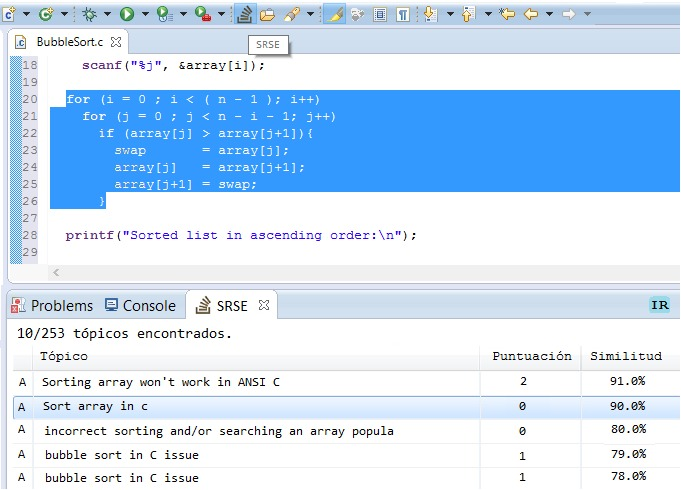
\includegraphics[width=0.8\linewidth]{srse}
\end{figure}
\end{frame}

\begin{frame}{Evaluación del Sistema de Recomendación}
\textbf{Conjunto 3:}
\begin{table}[h]
\caption{Resultados generales.}
\centering
\resizebox{\columnwidth}{!}{
\begin{tabular}{ccccc}
\hline
{Algoritmo} & {Resultado} & {Líneas} & {Candidatos} & {Porcentaje} \\
\hline
Alexander Bogomolny & $Encontrado$ & $36$ & $3$ & $83\%$ \\
Bin Packing & $No encontrado$ & $30$ & $6$ & $55\%$ \\
Binary Search Tree & $Encontrado$ & $163$ & $47$ & $64\%$ \\
Fibonacci Search & $No Encontrado$ & $48$ & $0$ & $0\%$ \\
Fisher Yates & $Encontrado$ & $33$ & $2$ & $63\%$ \\
Hash Table & $No Encontrado$ & $184$ & $0$ & $0\%$ \\
0-1 Knapsack Problem & $Encontrado$ & $78$ & $1$ & $94\%$ \\
Naor Reigngold & $No Encontrado$ & $17$ & $0$ & $0\%$ \\
Selection Sort & $Encontrado$ & $41$ & $6$ & $68\%$ \\
Sieve Eratosthenes & $Encontrado$ & $22$ & $2$ & $78\%$ \\
\hline
\end{tabular}
}
\end{table}
\end{frame}

\begin{frame}{Evaluación del Sistema de Recomendación}
\begin{table}[H]
\caption{Síntesis de Resultados}
\centering
\begin{tabular}{ccc}
\hline
{Resultado} & {Cantidad} & {Porcentaje} \\
\hline
$Encontrado$ & $6$ & $60.0\%$ \\
$No Encontrado$ & $4$ & $40.0\%$ \\
$Relacionado$ & $0$ & $0.0\%$ \\
\hline
\end{tabular}
\end{table}
\end{frame}

\begin{frame}{Conclusiones}
\begin{center}
``El sistema implementado demostró funcionar correctamente al sugerir tópicos con
fragmentos de código, iguales o similares al proporcionado por el usuario''
\end{center}
~

Resultados parciales:
\begin{itemize}
  \item El índice desarrollado es eficaz.
  \item Baja especificidad en los fragmentos de código.
\end{itemize}
\end{frame}

\begin{frame}{Recomendaciones}
\begin{itemize}
  \item Expandir el preprocesamiento.
  \item Ampliar el análisis sintáctico.
  \item Emplear función de \textit{hash} en el índice.
  \item Clasificación automática de los resultados.
  \item Algoritmos para evaluar contención de conjuntos.
\end{itemize}
\end{frame}

\end{document}